\documentclass{article}

% Packages required to support encoding
\usepackage{ucs}
\usepackage[utf8x]{inputenc}
\usepackage{graphicx} 
% Packages required by code

% Packages always used
\usepackage{listings}
\usepackage{hyperref}
\usepackage{xspace}
\usepackage[usenames,dvipsnames]{color}
\hypersetup{colorlinks=true,urlcolor=blue}


\usepackage[framed,numbered,autolinebreaks,useliterate] {mcode}


\usepackage{geometry}
\geometry{letterpaper,textwidth=350pt,textheight=680pt,tmargin=60pt,
            left=72pt,footskip=24pt,headsep=18pt,headheight=14pt}
\usepackage{amsmath}
\usepackage{amssymb}
\usepackage{textcase}
\usepackage{soul}

\newcommand{\mat}[1]{\boldsymbol{#1}}\renewcommand{\vec}[1]{\boldsymbol{\mathrm{#1}}}
\newcommand{\vecalt}[1]{\boldsymbol{#1}}

\newcommand{\conj}[1]{\overline{#1}}

\newcommand{\normof}[1]{\|#1\|}
\newcommand{\onormof}[2]{\|#1\|_{#2}}

\newcommand{\itr}[2]{#1^{(#2)}}
\newcommand{\itn}[1]{^{(#1)}}

\newcommand{\eps}{\varepsilon}
\newcommand{\kron}{\otimes}

\DeclareMathOperator{\diag}{diag}
\DeclareMathOperator{\trace}{trace}
\DeclareMathOperator{\tvec}{vec}

\newcommand{\prob}{\mathbb{P}}
\newcommand{\probof}[1]{\prob\left\{ #1 \right\}}

\newcommand{\pmat}[1]{\begin{pmatrix} #1 \end{pmatrix}}
\newcommand{\bmat}[1]{\begin{bmatrix} #1 \end{bmatrix}}
\newcommand{\spmat}[1]{\left(\begin{smallmatrix} #1 \end{smallmatrix}\right)}
\newcommand{\sbmat}[1]{\left[\begin{smallmatrix} #1 \end{smallmatrix}\right]}

\newcommand{\RR}{\mathbb{R}}
\newcommand{\CC}{\mathbb{C}}

\providecommand{\eye}{\mat{I}}
\providecommand{\mA}{\ensuremath{\mat{A}}}
\providecommand{\mB}{\ensuremath{\mat{B}}}
\providecommand{\mC}{\ensuremath{\mat{C}}}
\providecommand{\mD}{\ensuremath{\mat{D}}}
\providecommand{\mE}{\ensuremath{\mat{E}}}
\providecommand{\mF}{\ensuremath{\mat{F}}}
\providecommand{\mG}{\ensuremath{\mat{G}}}
\providecommand{\mH}{\ensuremath{\mat{H}}}
\providecommand{\mI}{\ensuremath{\mat{I}}}
\providecommand{\mJ}{\ensuremath{\mat{J}}}
\providecommand{\mK}{\ensuremath{\mat{K}}}
\providecommand{\mL}{\ensuremath{\mat{L}}}
\providecommand{\mM}{\ensuremath{\mat{M}}}
\providecommand{\mN}{\ensuremath{\mat{N}}}
\providecommand{\mO}{\ensuremath{\mat{O}}}
\providecommand{\mP}{\ensuremath{\mat{P}}}
\providecommand{\mQ}{\ensuremath{\mat{Q}}}
\providecommand{\mR}{\ensuremath{\mat{R}}}
\providecommand{\mS}{\ensuremath{\mat{S}}}
\providecommand{\mT}{\ensuremath{\mat{T}}}
\providecommand{\mU}{\ensuremath{\mat{U}}}
\providecommand{\mV}{\ensuremath{\mat{V}}}
\providecommand{\mW}{\ensuremath{\mat{W}}}
\providecommand{\mX}{\ensuremath{\mat{X}}}
\providecommand{\mY}{\ensuremath{\mat{Y}}}
\providecommand{\mZ}{\ensuremath{\mat{Z}}}
\providecommand{\mLambda}{\ensuremath{\mat{\Lambda}}}
\providecommand{\mPbar}{\bar{\mP}}

\providecommand{\ones}{\vec{e}}
\providecommand{\va}{\ensuremath{\vec{a}}}
\providecommand{\vb}{\ensuremath{\vec{b}}}
\providecommand{\vc}{\ensuremath{\vec{c}}}
\providecommand{\vd}{\ensuremath{\vec{d}}}
\providecommand{\ve}{\ensuremath{\vec{e}}}
\providecommand{\vf}{\ensuremath{\vec{f}}}
\providecommand{\vg}{\ensuremath{\vec{g}}}
\providecommand{\vh}{\ensuremath{\vec{h}}}
\providecommand{\vi}{\ensuremath{\vec{i}}}
\providecommand{\vj}{\ensuremath{\vec{j}}}
\providecommand{\vk}{\ensuremath{\vec{k}}}
\providecommand{\vl}{\ensuremath{\vec{l}}}
\providecommand{\vm}{\ensuremath{\vec{l}}}
\providecommand{\vn}{\ensuremath{\vec{n}}}
\providecommand{\vo}{\ensuremath{\vec{o}}}
\providecommand{\vp}{\ensuremath{\vec{p}}}
\providecommand{\vq}{\ensuremath{\vec{q}}}
\providecommand{\vr}{\ensuremath{\vec{r}}}
\providecommand{\vs}{\ensuremath{\vec{s}}}
\providecommand{\vt}{\ensuremath{\vec{t}}}
\providecommand{\vu}{\ensuremath{\vec{u}}}
\providecommand{\vv}{\ensuremath{\vec{v}}}
\providecommand{\vw}{\ensuremath{\vec{w}}}
\providecommand{\vx}{\ensuremath{\vec{x}}}
\providecommand{\vy}{\ensuremath{\vec{y}}}
\providecommand{\vz}{\ensuremath{\vec{z}}}
\providecommand{\vpi}{\ensuremath{\vecalt{\pi}}}

\sodef\allcapsspacing{\upshape}{0.15em}{0.65em}{0.6em}%

\makeatletter
\def\maketitle{%
\par
\hrule height 0.75pt\vspace{1ex}
\par\noindent
\begin{minipage}{0.5\textwidth}
\scshape
purdue university $\cdot$ CS 580 \\
Introduction to the Analysis of Algorithms
\end{minipage}
\begin{minipage}{0.5\textwidth}
\raggedleft
\MakeTextUppercase{\allcapsspacing{\@title}}\\[0.2ex]
\textit{\@author}\\[0.2ex]
\textit{\@date}
\end{minipage}
\par\vspace{1ex}
\hrule height 1pt
\vspace{2ex}
\par
}
\makeatother

\author{Jun Cheng}
\title{Lecture Notes}
% auto generate a title
\AtBeginDocument{\maketitle}


\title{Homework}



\begin{document} 



\hypertarget{problem_0_homework_checklist_2}{}
\subsection*{{Problem 0: Homework checklist}}
\label{problem_0_homework_checklist_2}

\checkmark	I didn't talk with any one about this homework. \newline
\checkmark 	Source-code are included at the end of this document. 

\hypertarget{}{}
\subsection*{{Problem 1:}}
\label{}
\begin{enumerate}

\item 
Function backsolve.m
\begin{lstlisting} 
function x = backsolve(A, b) 
    % Assume matrix A is n by n upper triangular matrix; 
    % Vector b is n by 1. 
    n = length(b) ;         %% Get the length of the vector b
    x = zeros(n,1);         %% initiate solution Xl 
    x(n) = b(n)/A(n,n);     %% For the base case, x(n) = b(n)/A(n,n); 
    for i=n-1:-1:1
        temp = 0;           
        for j = i:n 
            temp = temp + A(i, j)*x(j);    %% Accumulate all the other terms
        end 
        x(i) = (b(i)-temp)/A(i,i);    %%  solve X(i)
    end 
end
\end{lstlisting} 

Function forwardsolve.m: 
\begin{lstlisting} 
function x = forwardsolve(A, b) 
    % Assume matrix A is n by n upper triangular matrix; 
    % Vector b is n by 1. 
    n = length(b) ;         %% Get the length of the vector b
    x = zeros(n,1);         %% Initiate solution Xl 
    x(1) = b(1)/A(1,1);     %% For the base case, x(1) = b(1)/A(1,1); 
    for i=2:n
        temp = 0; 
        for j = 1:i 
            temp = temp + A(i, j)*x(j); %% Accumulate all the other terms
        end 
        x(i) = (b(i)-temp)/A(i,i);  %%  solve X(i)
    end 
end

\end{lstlisting} 

\item 
 
 I set $n=1000$ and repeat the procedure for 100 times. The time elapses for  Matlab backslash method is around $3.210974$ seconds.  My backsolve method will spend around $4.733596 $ seconds.  Matlab backslash has better performance than mine. 
 
 For the accuaracy: 
 \begin{align} 
\frac{ \|X_{matlab} - X_{mine} \| }{\|X_{matlab} \| }=  7.2165e-16
 \end{align} 
 
\item My linear solver function: \\
\begin{lstlisting} 
function x = linearSolver(A, b)     
    [L, U, P] = lu(A);
    x1 = forwardsolve(L, P*b); 
    x = backsolve(U, x1); 
end 
\end{lstlisting} 

\begin{figure}
\centering
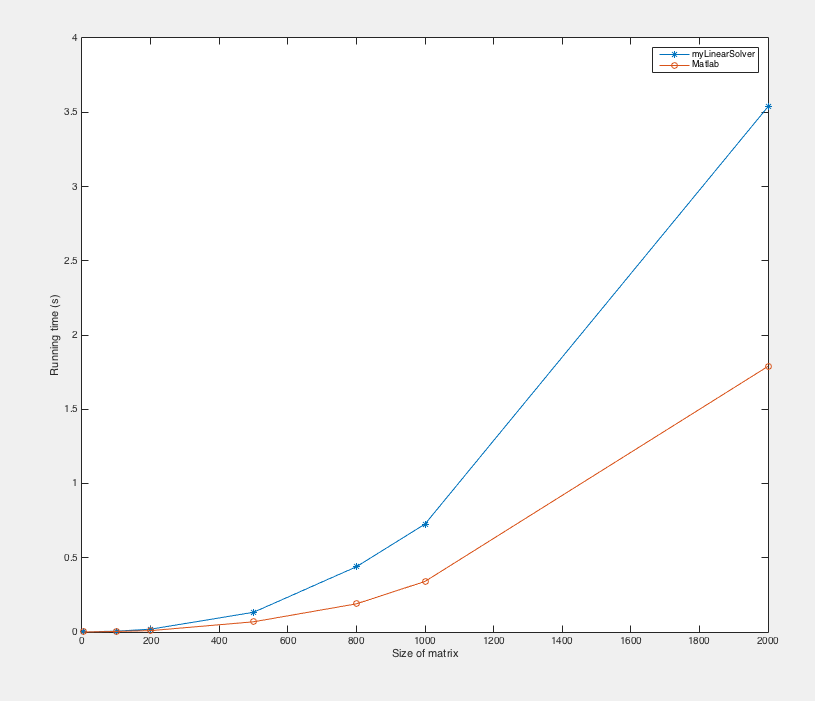
\includegraphics[width=0.8\textwidth]{time}
\caption{Time consumption for different size of matrix.}
\end{figure}

\begin{figure}
\centering
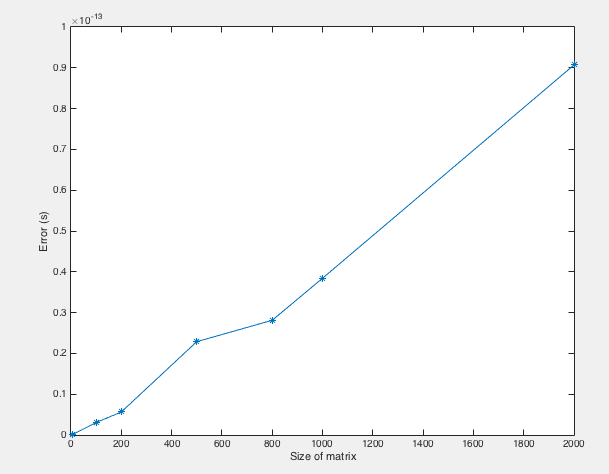
\includegraphics[width=0.8\textwidth]{error}
\caption{Error plot between Matlab backslash solver and my linear solver.}
\end{figure}

\end{enumerate}



\hypertarget{}{}
\subsection*{{Problem 2:}}
\label{}
\begin{enumerate}
\item 
Base on \begin{align*}  \frac{1}{h^2}(u(x_{i-1}, y_j) + u(x_i,y_{j-1})-4u(x_i,y_j)+u(x_{i+1},y_j)+u(x_i,y_{j+1}))=f(x_i,y_j)    \end{align*}

Then all the linear equations: 
\begin{align*}
(i=0, j=0): & f_{0,0} =0\\
(i=0, j=1): & f_{0,1} =0\\
(i=0, j=2): & f_{0,2} =0\\
(i=0, j=3): & f_{0,3} =0\\
(i=1, j=0): & f_{1,0} =0\\
(i=1, j=1): & f_{1,1} =0\\
(i=1, j=2): & f_{1,2} =0\\
(i=1, j=3): & f_{1,3} =0\\
(i=2, j=0): & f_{2,0} =0\\
(i=2, j=1): & f_{2,1} =0\\
(i=3, j=0): & f_{3,0} =0\\
(i=3, j=1): & f_{3,1} =0\\
\end{align*} 
All the others:  \begin{align*}
(i=2, j=2): & f_{2,2} =\frac{1}{h^2}(u(x_{1}, y_2) + u(x_2,y_{1})-4u(x_2,y_2)+u(x_{3},y_2)+u(x_2,y_{3}))\\
(i=2, j=3): & f_{2,3} =\frac{1}{h^2}(u(x_{1}, y_3) + u(x_2,y_{2})-4u(x_2,y_3)+u(x_{3},y_3)+u(x_2,y_{3}))\\
(i=3, j=2): & f_{3,2} =\frac{1}{h^2}(u(x_{2}, y_2) + u(x_3,y_{2})-4u(x_3,y_2)+u(x_{4},y_2)+u(x_3,y_{3})) \\
(i=3, j=3): & f_{3,3} =\frac{1}{h^2}(u(x_{2}, y_3) + u(x_2,y_{2})-4u(x_3,y_3)+u(x_{4},y_3)+u(x_3,y_{4})) \\
\end{align*} 
\item 
The code is filled as below: 
\begin{lstlisting}
n = 10;
A = zeros((n+1)^2,(n+1)^2);
newA = zeros((n+1)^2-2, (n+1)^2-2); 
f = zeros((n+1)^2,1);
G = reshape(1:((n+1)^2), n+1, n+1)'; 
for i=0:n
 for j=0:n
     row = G(i+1,j+1);
     if i==0 || j == 0 || i==n || j==n
         % we are on a boundary
         f(row) = 0;
         A(row, row) = 1;     % For boundary points, we set the diagonal term to be 1. 
        
     else
         % we are NOT on a boundary
         f(row) = 1/n^2;
            A(row, G(i,j+1  )) = 1;             % Put the coefficients to the corresponding entry of matrix A. 
            A(row, G(i+1,  j)) = 1; 
            A(row, G(i+1,  j+1  )) = -4; 
            A(row, G(i+2,j+1  )) = 1 ; 
            A(row, G(i+1,  j+2)) = 1; 
        % end
            
     end
 end
end
u = A\f;
\end{lstlisting}


\item 
Using Matlab's backslash solver, I can get the result for $u$ : \\
\begingroup
\fontsize{8pt}{12pt}\selectfont
\begin{verbatim}
0         0         0         0         0         0         0         0         0         0         0
0   -0.0128   -0.0206   -0.0254   -0.0280   -0.0288   -0.0280   -0.0254   -0.0206   -0.0128         0
0   -0.0206   -0.0343   -0.0430   -0.0478   -0.0493   -0.0478   -0.0430   -0.0343   -0.0206         0
0   -0.0254   -0.0430   -0.0544   -0.0608   -0.0629   -0.0608   -0.0544   -0.0430   -0.0254         0
0   -0.0280   -0.0478   -0.0608   -0.0682   -0.0706   -0.0682   -0.0608   -0.0478   -0.0280         0
0   -0.0288   -0.0493   -0.0629   -0.0706   -0.0731   -0.0706   -0.0629   -0.0493   -0.0288         0
0   -0.0280   -0.0478   -0.0608   -0.0682   -0.0706   -0.0682   -0.0608   -0.0478   -0.0280         0
0   -0.0254   -0.0430   -0.0544   -0.0608   -0.0629   -0.0608   -0.0544   -0.0430   -0.0254         0
0   -0.0206   -0.0343   -0.0430   -0.0478   -0.0493   -0.0478   -0.0430   -0.0343   -0.0206         0
0   -0.0128   -0.0206   -0.0254   -0.0280   -0.0288   -0.0280   -0.0254   -0.0206   -0.0128         0
0         0         0         0         0         0         0         0         0         0         0
\end{verbatim}
\endgroup



\end{enumerate} 


\hypertarget{}{}
\subsection*{{Problem 3: The Schur Complement}}
\label{}

\begin{enumerate} 
\item 
\begin{align*} 
\mC \vx_1+\mD \vx_2 & = \vb_2\\
\mD \vx_2 & = \vb_2-\mC \vx_1 \\
\vx_2 & = \mD^{-1}(\vb_2- \mC \vx_1) \\
\end{align*}
It is possible when the block matrix $\mD$ is invertible because we need the inverse of matrix $\mD$. \\

\item 
\begin{align*}
\mA\vx_1+\mB\vx_2=\vb_1\\
\mC\vx_1+\mD\vx_2=\vb_2 \\
\end{align*}
Now we know that $\mD$ is invertible. So multiply $\mB\mD^{-1}$ on the second equation: 
\begin{align*}
\mA\vx_1+\mB\vx_2 &=\vb_1\\
\mB\mD^{-1}\mC\vx_1+\mB\vx_2 &=\mB\mD^{-1}\vb_2 \\
(\mB\mD^{-1}\mC -\mA )\vx_1&= (\mB\mD^{-1}\vb_2- \vb_1)
\end{align*}
So if we can get inverse of $ \mB\mD^{-1}\mC -\mA $, then we can solve $\vx_1$.
\item 
Then we can solve \begin{align*}
\vx_1 = (\mB\mD^{-1}\mC -\mA )^{-1}(\mB\mD^{-1}\vb_2- \vb_1)\\
\end{align*}
\end{enumerate} 


\begin{figure}
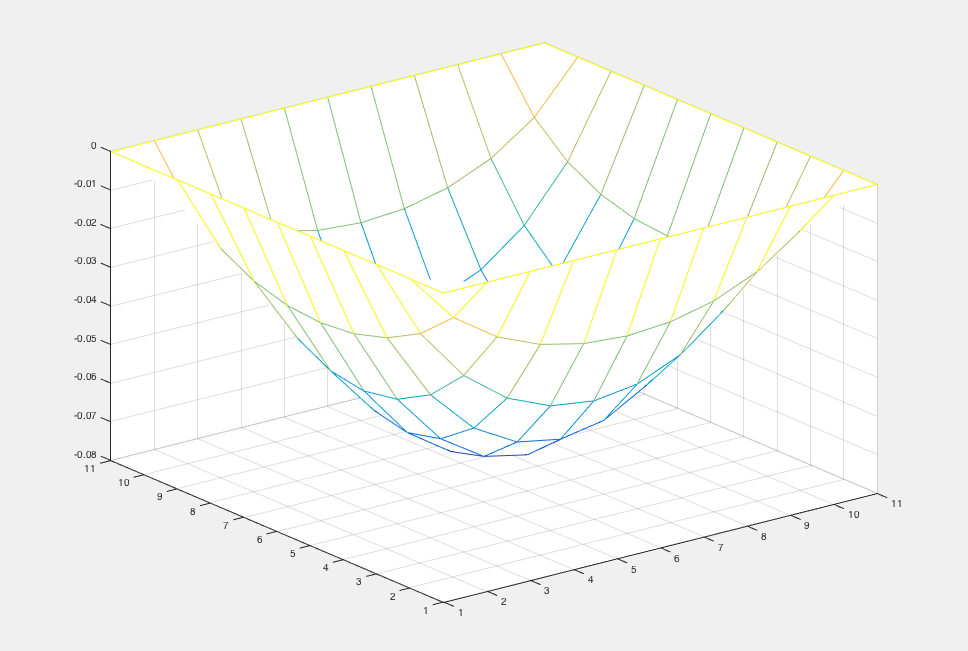
\includegraphics[width=0.7\textwidth]{meshplot} 
\centering
\caption{Surface plot of $\mu$. } 
\end{figure}

\hypertarget{}{}
\subsection*{{Problem 4:Ranking with Linear Systems}}
\label{}
Questions: \\
I am a little confuse why we need ${r_1, r_2, ..., r_n} $ to be the indicate the performance of each team, instead of  ${S_1, S_2, ..., S_n} $? \\





\end{document}
